\documentclass[twoside]{book}

% Packages required by doxygen
\usepackage{fixltx2e}
\usepackage{calc}
\usepackage{doxygen}
\usepackage[export]{adjustbox} % also loads graphicx
\usepackage{graphicx}
\usepackage[utf8]{inputenc}
\usepackage{makeidx}
\usepackage{multicol}
\usepackage{multirow}
\PassOptionsToPackage{warn}{textcomp}
\usepackage{textcomp}
\usepackage[nointegrals]{wasysym}
\usepackage[table]{xcolor}

% Font selection
\usepackage[T1]{fontenc}
\usepackage[scaled=.90]{helvet}
\usepackage{courier}
\usepackage{amssymb}
\usepackage{sectsty}
\renewcommand{\familydefault}{\sfdefault}
\allsectionsfont{%
  \fontseries{bc}\selectfont%
  \color{darkgray}%
}
\renewcommand{\DoxyLabelFont}{%
  \fontseries{bc}\selectfont%
  \color{darkgray}%
}
\newcommand{\+}{\discretionary{\mbox{\scriptsize$\hookleftarrow$}}{}{}}

% Page & text layout
\usepackage{geometry}
\geometry{%
  a4paper,%
  top=2.5cm,%
  bottom=2.5cm,%
  left=2.5cm,%
  right=2.5cm%
}
\tolerance=750
\hfuzz=15pt
\hbadness=750
\setlength{\emergencystretch}{15pt}
\setlength{\parindent}{0cm}
\setlength{\parskip}{3ex plus 2ex minus 2ex}
\makeatletter
\renewcommand{\paragraph}{%
  \@startsection{paragraph}{4}{0ex}{-1.0ex}{1.0ex}{%
    \normalfont\normalsize\bfseries\SS@parafont%
  }%
}
\renewcommand{\subparagraph}{%
  \@startsection{subparagraph}{5}{0ex}{-1.0ex}{1.0ex}{%
    \normalfont\normalsize\bfseries\SS@subparafont%
  }%
}
\makeatother

% Headers & footers
\usepackage{fancyhdr}
\pagestyle{fancyplain}
\fancyhead[LE]{\fancyplain{}{\bfseries\thepage}}
\fancyhead[CE]{\fancyplain{}{}}
\fancyhead[RE]{\fancyplain{}{\bfseries\leftmark}}
\fancyhead[LO]{\fancyplain{}{\bfseries\rightmark}}
\fancyhead[CO]{\fancyplain{}{}}
\fancyhead[RO]{\fancyplain{}{\bfseries\thepage}}
\fancyfoot[LE]{\fancyplain{}{}}
\fancyfoot[CE]{\fancyplain{}{}}
\fancyfoot[RE]{\fancyplain{}{\bfseries\scriptsize Generated by Doxygen }}
\fancyfoot[LO]{\fancyplain{}{\bfseries\scriptsize Generated by Doxygen }}
\fancyfoot[CO]{\fancyplain{}{}}
\fancyfoot[RO]{\fancyplain{}{}}
\renewcommand{\footrulewidth}{0.4pt}
\renewcommand{\chaptermark}[1]{%
  \markboth{#1}{}%
}
\renewcommand{\sectionmark}[1]{%
  \markright{\thesection\ #1}%
}

% Indices & bibliography
\usepackage{natbib}
\usepackage[titles]{tocloft}
\setcounter{tocdepth}{3}
\setcounter{secnumdepth}{5}
\makeindex

% Hyperlinks (required, but should be loaded last)
\usepackage{ifpdf}
\ifpdf
  \usepackage[pdftex,pagebackref=true]{hyperref}
\else
  \usepackage[ps2pdf,pagebackref=true]{hyperref}
\fi
\hypersetup{%
  colorlinks=true,%
  linkcolor=blue,%
  citecolor=blue,%
  unicode%
}

% Custom commands
\newcommand{\clearemptydoublepage}{%
  \newpage{\pagestyle{empty}\cleardoublepage}%
}

\usepackage{caption}
\captionsetup{labelsep=space,justification=centering,font={bf},singlelinecheck=off,skip=4pt,position=top}

%===== C O N T E N T S =====

\begin{document}

% Titlepage & ToC
\hypersetup{pageanchor=false,
             bookmarksnumbered=true,
             pdfencoding=unicode
            }
\pagenumbering{alph}
\begin{titlepage}
\vspace*{7cm}
\begin{center}%
{\Large pi-\/openvg-\/knobs }\\
\vspace*{1cm}
{\large Generated by Doxygen 1.8.13}\\
\end{center}
\end{titlepage}
\clearemptydoublepage
\pagenumbering{roman}
\tableofcontents
\clearemptydoublepage
\pagenumbering{arabic}
\hypersetup{pageanchor=true}

%--- Begin generated contents ---
\chapter{Main Page}
\label{index}\hypertarget{index}{}This is a raspberry pi application.

Creates shapes using openvg.

It requires the ajstarks library and other installation as described here\+: \href{https://github.com/ajstarks/openvg/blob/master/README.md#build-and-run}{\tt https\+://github.\+com/ajstarks/openvg/blob/master/\+R\+E\+A\+D\+M\+E.\+md\#build-\/and-\/run}

doxygen\+: \href{https://brathke.github.io/pi-openvg-knobs/html/index.html}{\tt https\+://brathke.\+github.\+io/pi-\/openvg-\/knobs/html/index.\+html} 
\chapter{File Index}
\section{File List}
Here is a list of all files with brief descriptions\+:\begin{DoxyCompactList}
\item\contentsline{section}{\hyperlink{pi-openvg-knobs_8c}{pi-\/openvg-\/knobs.\+c} }{\pageref{pi-openvg-knobs_8c}}{}
\end{DoxyCompactList}

\chapter{File Documentation}
\hypertarget{pi-openvg-knobs_8c}{}\section{pi-\/openvg-\/knobs.c File Reference}
\label{pi-openvg-knobs_8c}\index{pi-\/openvg-\/knobs.\+c@{pi-\/openvg-\/knobs.\+c}}
{\ttfamily \#include $<$stdio.\+h$>$}\newline
{\ttfamily \#include $<$stdlib.\+h$>$}\newline
{\ttfamily \#include $<$unistd.\+h$>$}\newline
{\ttfamily \#include \char`\"{}V\+G/openvg.\+h\char`\"{}}\newline
{\ttfamily \#include \char`\"{}V\+G/vgu.\+h\char`\"{}}\newline
{\ttfamily \#include \char`\"{}fontinfo.\+h\char`\"{}}\newline
{\ttfamily \#include \char`\"{}shapes.\+h\char`\"{}}\newline
{\ttfamily \#include $<$signal.\+h$>$}\newline
{\ttfamily \#include $<$math.\+h$>$}\newline
Include dependency graph for pi-\/openvg-\/knobs.c\+:\nopagebreak
\begin{figure}[H]
\begin{center}
\leavevmode
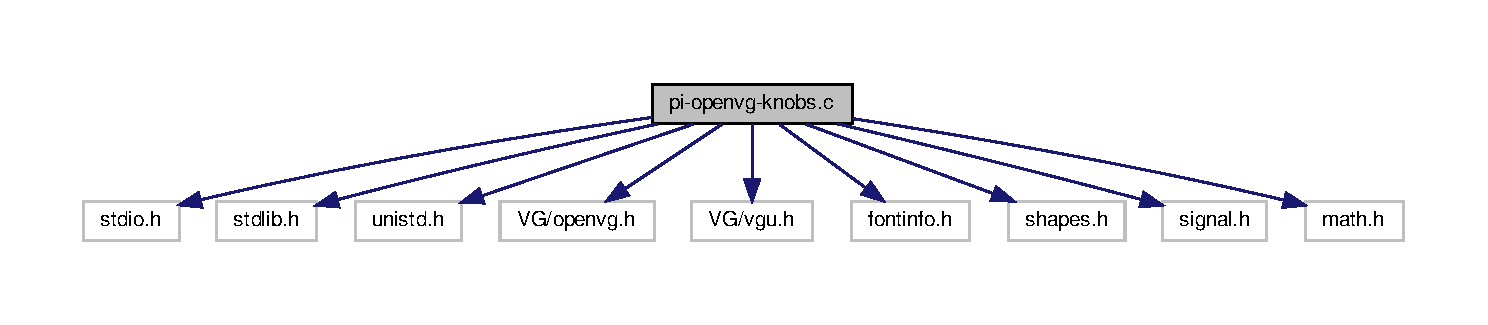
\includegraphics[width=350pt]{pi-openvg-knobs_8c__incl}
\end{center}
\end{figure}
\subsection*{Functions}
\begin{DoxyCompactItemize}
\item 
void \hyperlink{pi-openvg-knobs_8c_a358d026c8b5c38a548bac21e2e279719}{draw} (int width, int height)
\item 
void \hyperlink{pi-openvg-knobs_8c_a5054c36923934387c6f7605dd1a2f3c9}{sig\+\_\+handler} (int sig)
\item 
int \hyperlink{pi-openvg-knobs_8c_a3c04138a5bfe5d72780bb7e82a18e627}{main} (int argc, char $\ast$$\ast$argv)
\end{DoxyCompactItemize}


\subsection{Function Documentation}
\mbox{\Hypertarget{pi-openvg-knobs_8c_a358d026c8b5c38a548bac21e2e279719}\label{pi-openvg-knobs_8c_a358d026c8b5c38a548bac21e2e279719}} 
\index{pi-\/openvg-\/knobs.\+c@{pi-\/openvg-\/knobs.\+c}!draw@{draw}}
\index{draw@{draw}!pi-\/openvg-\/knobs.\+c@{pi-\/openvg-\/knobs.\+c}}
\subsubsection{\texorpdfstring{draw()}{draw()}}
{\footnotesize\ttfamily void draw (\begin{DoxyParamCaption}\item[{int}]{width,  }\item[{int}]{height }\end{DoxyParamCaption})}



Definition at line 11 of file pi-\/openvg-\/knobs.\+c.

Here is the caller graph for this function\+:\nopagebreak
\begin{figure}[H]
\begin{center}
\leavevmode
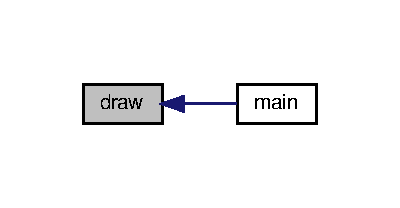
\includegraphics[width=192pt]{pi-openvg-knobs_8c_a358d026c8b5c38a548bac21e2e279719_icgraph}
\end{center}
\end{figure}
\mbox{\Hypertarget{pi-openvg-knobs_8c_a3c04138a5bfe5d72780bb7e82a18e627}\label{pi-openvg-knobs_8c_a3c04138a5bfe5d72780bb7e82a18e627}} 
\index{pi-\/openvg-\/knobs.\+c@{pi-\/openvg-\/knobs.\+c}!main@{main}}
\index{main@{main}!pi-\/openvg-\/knobs.\+c@{pi-\/openvg-\/knobs.\+c}}
\subsubsection{\texorpdfstring{main()}{main()}}
{\footnotesize\ttfamily int main (\begin{DoxyParamCaption}\item[{int}]{argc,  }\item[{char $\ast$$\ast$}]{argv }\end{DoxyParamCaption})}



Definition at line 66 of file pi-\/openvg-\/knobs.\+c.

Here is the call graph for this function\+:\nopagebreak
\begin{figure}[H]
\begin{center}
\leavevmode
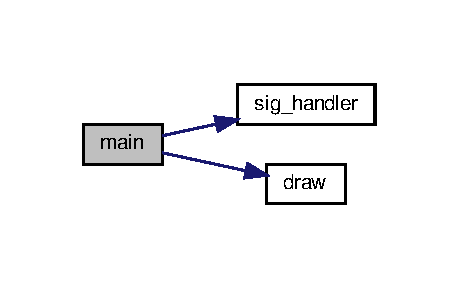
\includegraphics[width=220pt]{pi-openvg-knobs_8c_a3c04138a5bfe5d72780bb7e82a18e627_cgraph}
\end{center}
\end{figure}
\mbox{\Hypertarget{pi-openvg-knobs_8c_a5054c36923934387c6f7605dd1a2f3c9}\label{pi-openvg-knobs_8c_a5054c36923934387c6f7605dd1a2f3c9}} 
\index{pi-\/openvg-\/knobs.\+c@{pi-\/openvg-\/knobs.\+c}!sig\+\_\+handler@{sig\+\_\+handler}}
\index{sig\+\_\+handler@{sig\+\_\+handler}!pi-\/openvg-\/knobs.\+c@{pi-\/openvg-\/knobs.\+c}}
\subsubsection{\texorpdfstring{sig\+\_\+handler()}{sig\_handler()}}
{\footnotesize\ttfamily void sig\+\_\+handler (\begin{DoxyParamCaption}\item[{int}]{sig }\end{DoxyParamCaption})}



Definition at line 60 of file pi-\/openvg-\/knobs.\+c.

Here is the caller graph for this function\+:\nopagebreak
\begin{figure}[H]
\begin{center}
\leavevmode
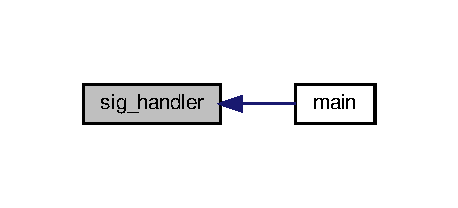
\includegraphics[width=220pt]{pi-openvg-knobs_8c_a5054c36923934387c6f7605dd1a2f3c9_icgraph}
\end{center}
\end{figure}

\hypertarget{_r_e_a_d_m_e_8md}{}\section{R\+E\+A\+D\+M\+E.\+md File Reference}
\label{_r_e_a_d_m_e_8md}\index{R\+E\+A\+D\+M\+E.\+md@{R\+E\+A\+D\+M\+E.\+md}}

%--- End generated contents ---

% Index
\backmatter
\newpage
\phantomsection
\clearemptydoublepage
\addcontentsline{toc}{chapter}{Index}
\printindex

\end{document}
